\documentclass[10pt,a4paper]{article}
\usepackage[utf8]{inputenc}
\usepackage{graphicx}
\usepackage[french]{babel}
\frenchbsetup{StandardLists=true}
\usepackage{color}
\usepackage{amsmath} 
\usepackage{eso-pic} 
\usepackage{algpseudocode}
\usepackage[T1]{fontenc}

\usepackage{xcolor}
\usepackage{listings}
\lstset{
literate=
{á}{{\'a}}1 {é}{{\'e}}1 {í}{{\'i}}1 {ó}{{\'o}}1 {ú}{{\'u}}1
{Á}{{\'A}}1 {É}{{\'E}}1 {Í}{{\'I}}1 {Ó}{{\'O}}1 {Ú}{{\'U}}1
{à}{{\`a}}1 {è}{{\`e}}1 {ì}{{\`i}}1 {ò}{{\`o}}1 {ù}{{\`u}}1
{À}{{\`A}}1 {È}{{\'E}}1 {Ì}{{\`I}}1 {Ò}{{\`O}}1 {Ù}{{\`U}}1
{ä}{{\"a}}1 {ë}{{\"e}}1 {ï}{{\"i}}1 {ö}{{\"o}}1 {ü}{{\"u}}1
{Ä}{{\"A}}1 {Ë}{{\"E}}1 {Ï}{{\"I}}1 {Ö}{{\"O}}1 {Ü}{{\"U}}1
{â}{{\^a}}1 {ê}{{\^e}}1 {î}{{\^i}}1 {ô}{{\^o}}1 {û}{{\^u}}1
{Â}{{\^A}}1 {Ê}{{\^E}}1 {Î}{{\^I}}1 {Ô}{{\^O}}1 {Û}{{\^U}}1
{œ}{{\oe}}1 {Œ}{{\OE}}1 {æ}{{\ae}}1 {Æ}{{\AE}}1 {ß}{{\ss}}1
{ű}{{\H{u}}}1 {Ű}{{\H{U}}}1 {ő}{{\H{o}}}1 {Ő}{{\H{O}}}1
{ç}{{\c c}}1 {Ç}{{\c C}}1 {ø}{{\o}}1 {å}{{\r a}}1 {Å}{{\r A}}1
{€}{{\EUR}}1 {£}{{\pounds}}1
}
\lstdefinestyle{stylepython}{
 language=Python,
 basicstyle=\ttfamily,
 commentstyle=\color{green},
 keywordstyle=\color{blue},
 stringstyle=\color{olive},
 numberstyle=\tiny, 
 numbers=left,
 stepnumber=1, 
 numbersep=5pt
}

\usepackage{fancyhdr}
\pagestyle{fancy}

\fancyhf{}
 
\lfoot{}
\cfoot{}
\rfoot{}
 
\fancypagestyle{plain}{%
\fancyhf{} % clear all header and footer fields
\fancyfoot[L]{}
\fancyfoot[C]{}
\fancyfoot[R]{} %
}

\renewcommand{\headrulewidth}{1pt}
\fancyhead[R]{\textbf{page \thepage}} 
\fancyhead[L]{\leftmark}

\renewcommand{\footrulewidth}{1pt}
\fancyfoot[L]{\textbf{page \thepage}} 
\fancyfoot[R]{\leftmark}




\newcommand{\blap}[1]{\vbox to 0pt{#1\vss}}
\newcommand\AtUpperLeftCorner[3]{%
  \put(\LenToUnit{#1},\LenToUnit{\dimexpr\paperheight-#2}){\blap{#3}}%
} 
\newcommand\AtTopCenterPage[2]{%
  \put(\LenToUnit{.5\paperwidth},\LenToUnit{\dimexpr\paperheight-#1}){\blap{\hbox to 0pt{\hss#2\hss}}}%
} 
\newcommand\AtUpperRightCorner[3]{%
  \put(\LenToUnit{\dimexpr\paperwidth-#1},\LenToUnit{\dimexpr\paperheight-#2}){\blap{\llap{#3}}}%
}     

\title{Théorie du chaos}
\author{\textsc{Ben Brahim} Wilfried\\L1 Informatique\\2021/2022\\}
\date{\today}
\makeatletter        


\begin{document}
\begin{titlepage}
    \enlargethispage{2cm}
 
    \AddToShipoutPicture{
        \AtUpperLeftCorner{1.5cm}{1cm}{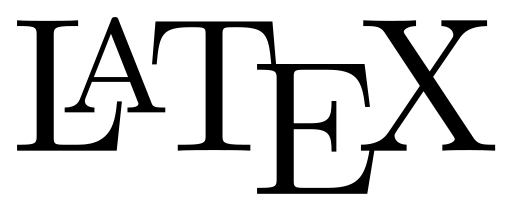
\includegraphics[width=6cm]{LaTeX_logo.svg.png}}
        \AtUpperRightCorner{1.5cm}{1cm}{
\includegraphics[width=6cm]{logop8-2.png}}
    }
    
    \vspace*{1cm}
	
	\begin{center}
        \makebox[\textwidth]{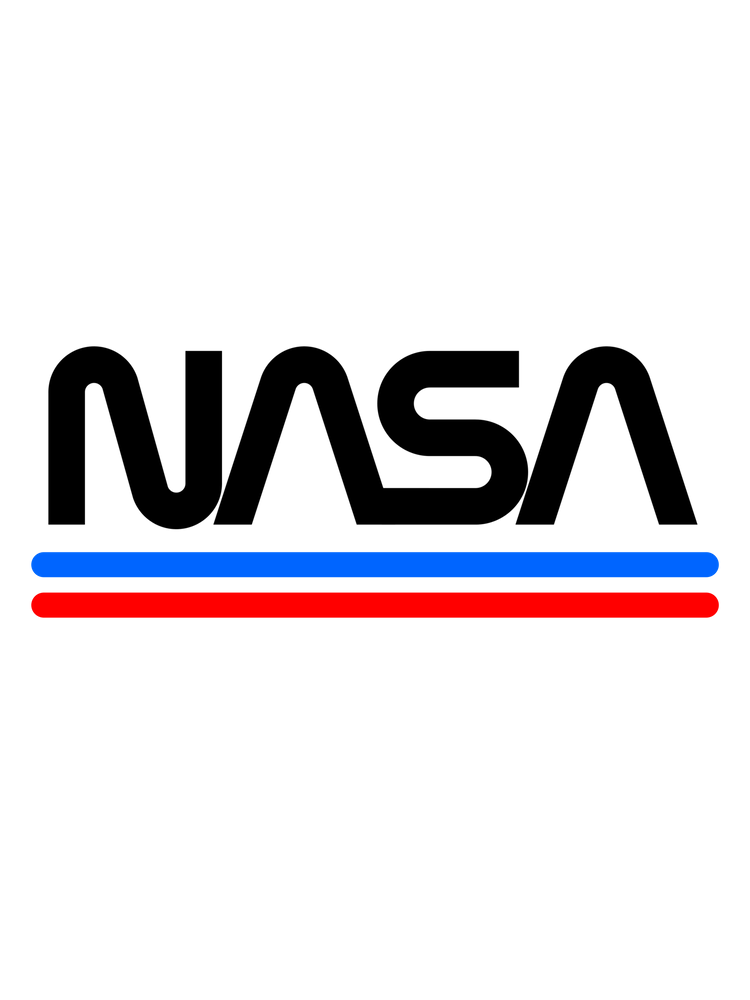
\includegraphics[width=12cm]{nasaa.png}}
    \end{center} 
 
    \begin{center}
        \large{\@title}
        \large{\@author}
        \large{\@date} 
    \end{center}

\end{titlepage}
\ClearShipoutPicture


\tableofcontents
\listoffigures
\listoftables

\section{Introduction a la théorie du chaos}
\subsection{Le système chaotique}

Un système dynamique est dit chaotique si une portion « significative » de son espace des phases présente simultanément les deux caractéristiques suivantes :

\begin{itemize}
\item le phénomène de sensibilité aux conditions initiales,
\item une forte récurrence.
\end{itemize}

La présence de ces deux propriétés entraîne un comportement extrêmement désordonné, qualifié à juste titre de « chaotique ». Les systèmes chaotiques s'opposent notamment aux systèmes intégrables de la mécanique classique, qui furent longtemps les symboles d'une régularité toute puissante en physique théorique. La dynamique quasi périodique d'un système intégrable semblait elle-même trouver son illustration parfaite dans les majestueux mouvements des planètes du Système solaire autour du Soleil ; aussi Voltaire, qui incita Émilie du Châtelet à entreprendre la traduction des Philosophiae naturalis principia mathematica de Newton, parlait de Dieu comme du « Grand Horloger »…

\subsection{Qu'est-ce que la « théorie du chaos » ?}

La théorie du chaos est un domaine de la dynamique déterministe qui avance que des éléments en apparence aléatoires peuvent résulter d'équations normales du fait de la complexité du système impliqué. En informatique, la théorie du chaos s'applique à de nombreux domaines notamment les réseaux, l'analytique du Big Data, la logique floue, l'informatique décisionnelle (BI, Business Intelligence), le marketing, la théorie des jeux, la pensée systémique, l'analytique prédictive et les réseaux sociaux.\vspace{0.40cm}

En mathématiques, la théorie du chaos étudie le comportement des systèmes dynamiques très sensibles aux conditions initiales, un phénomène généralement illustré par l'effet papillon.\vspace{0.40cm}

La théorie du chaos est une véritable théorie scientifique. Elle repose sur la représentation des solutions des équations différentielles dans l'espace des phases associé : représenter les solutions sous forme de trajectoire dans l'espace plutôt que l'une des variables en fonction du temps permet de révéler la structure sous-jacente : c'est ce qui conduit à affirmer que la théorie du chaos contribue à «trouver de l'ordre caché sous un désordre apparent.». L'attracteur de Lorenz précédemment représenté est un exemple d'une évolution d'un système dans l'espace des phases. Au déterminisme laplacien permettant la prédiction sur des temps arbitrairement longs a succédé un déterminisme de nature fondamentalement différente. Il peut être approché de manière probabiliste8 et alors caractérisé par l'existence d'invariants prenant la forme de mesures de probabilités, de dimension fractale… ou par une description topologique des attracteurs. Toutes les sciences, y compris sociales, sont concernées par ce changement de paradigme ; en particulier, cette théorie peut inclure l'organisation du vivant dans la nature.

\begin{figure}
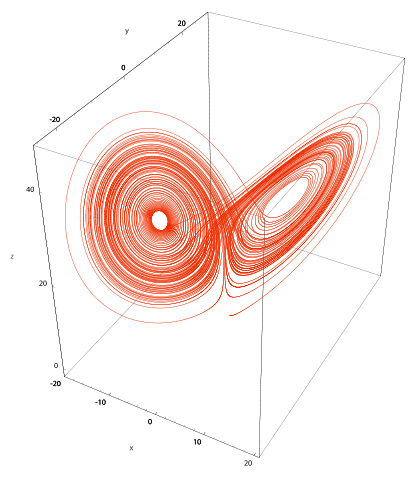
\includegraphics[width=9cm]{Lorenz_attractor_boxed.png}
\caption{Attracteur étrange de Lorenz (1963)}
\end{figure}
\newpage 

\section{Le déterminisme, de Laplace à Poincaré}

\subsection{La stabilité du Système solaire}

Le point de départ de la théorie du chaos est le problème à « 3 corps » qui consiste à étudier le mouvement de trois corps en interaction gravitationnelle, comme le système : { Soleil - Terre - Lune }, supposé isolé du reste de l'univers. Le but de cette recherche est de déterminer si le Système solaire est « stable » sur le long terme, ou bien si l'un des corps risque un jour de percuter un autre corps, ou encore être éjecté du Système solaire vers l'infini.\vspace{0.40cm}

Le problème à 3 corps est aussi vieux que la mécanique newtonienne ; en effet, dès la naissance de cette théorie, son fondateur s'est intéressé au problème à trois corps dans le but de prédire le mouvement de la Lune. Tous les astronomes à sa suite ont abordé ce problème, dont Laplace, qui crut avoir prouvé la stabilité du Système solaire en utilisant la théorie des perturbations au premier ordre. Malheureusement, le développement perturbatif au premier ordre est insuffisant pour conclure définitivement. Un siècle après Laplace, Henri Poincaré s'est donc emparé du problème. On examine ci-dessous l'évolution des idées qui distinguent la pensée de Laplace de celle de Poincaré.

\subsection{Notion de système dynamique différentiel conservatif}
Pour un système possédant n degrés de libertés, l'espace des phases ${\displaystyle \Gamma }$ du système possède 2n dimensions, de telle sorte que l'état complet ${\displaystyle x(t)\in \Gamma }$ du système à l'instant t est en général un vecteur à 2n composantes. On considère alors typiquement un système différentiel du premier ordre du type :\vspace{0.40cm}

\begin{math}
{\frac {dx(t)}{dt}}\ =\ f(x(t),t)\vspace{0.40cm}
\end{math}

où la fonction f définit le système dynamique étudié (c'est en général également un vecteur à n dimensions, c’est-à-dire un ensemble de n fonctions scalaires). Ce système physique, supposé conservatif, est déterministe si et seulement si la dynamique du système associe à chaque condition initiale ${\displaystyle x_{0}}$ un et un seul état final ${\displaystyle x(t)}$. Il faut pour cela qu'il existe une application bijective ${\displaystyle \phi _{t}:\Gamma \to \Gamma }\phi _{t}:\Gamma \to \Gamma$  de l'espace des phases sur lui-même telle que :\vspace{0.40cm}

\begin{math}
x(t)\ =\ \phi _{t}(x_{0})\vspace{0.40cm}
\end{math}

Lorsque le temps t varie, cette bijection engendre un flot sur ${\displaystyle \Gamma }$ , c’est-à-dire un groupe continu à un paramètre ${\displaystyle \phi _{t}}$. Cette modélisation mathématique correspond par exemple au flot hamiltonien de la mécanique classique, ainsi qu'au flot géodésique.

\newpage
\section{Attracteur de Lorenz algorithme python}
\begin{lstlisting}[style=stylepython]
import numpy as np
import matplotlib.pyplot as plt
from mpl_toolkits.mplot3d import Axes3D
prandtl = 10 
rho = 28
beta = 8/3
def lorenz_attr(x, y, z):
    x_dot = prandtl*(y - x)
    y_dot = rho*x - y - x*z
    z_dot = x*y - beta*z
    return x_dot, y_dot, z_dot
dt = 0.01
num_steps = 10000

xs = np.empty(num_steps + 1)
ys = np.empty(num_steps + 1)
zs = np.empty(num_steps + 1)
xs[0], ys[0], zs[0] = (0., 1., 1.05)
for i in range(num_steps):
    x_dot, y_dot, z_dot = lorenz_attr(xs[i], ys[i], zs[i])
    xs[i + 1] = xs[i] + (x_dot * dt)
    ys[i + 1] = ys[i] + (y_dot * dt)
    zs[i + 1] = zs[i] + (z_dot * dt)
fig = plt.figure()
ax = fig.gca(projection='3d')

ax.plot(xs, ys, zs, lw=0.5)
ax.set_xlabel("X Axis")
ax.set_ylabel("Y Axis")
ax.set_zlabel("Z Axis")
ax.set_title("Lorenz Attractor")

plt.show()
\end{lstlisting}

\section{Reference Bibliographique}
\begin{thebibliography}{1}
    \bibitem{C}
    James Gleick, La Théorie du chaos, 29 octobre 1987.
\end{thebibliography}


\end{document}
